\subsection{Overview and Control Objective}
\label{sec:objective}

\begin{figure*}[!t]
  \centering
  % Source PDF is 864.0 x 297.36 pt; measured ink box is x 21.1--854.9, y 12.5--285.8.
  % Trim removes the empty top/bottom bands and the 12 pt of excess left slack so the
  % remaining side margins match at 9.1 pt. Re-measure if the figure is re-exported.
  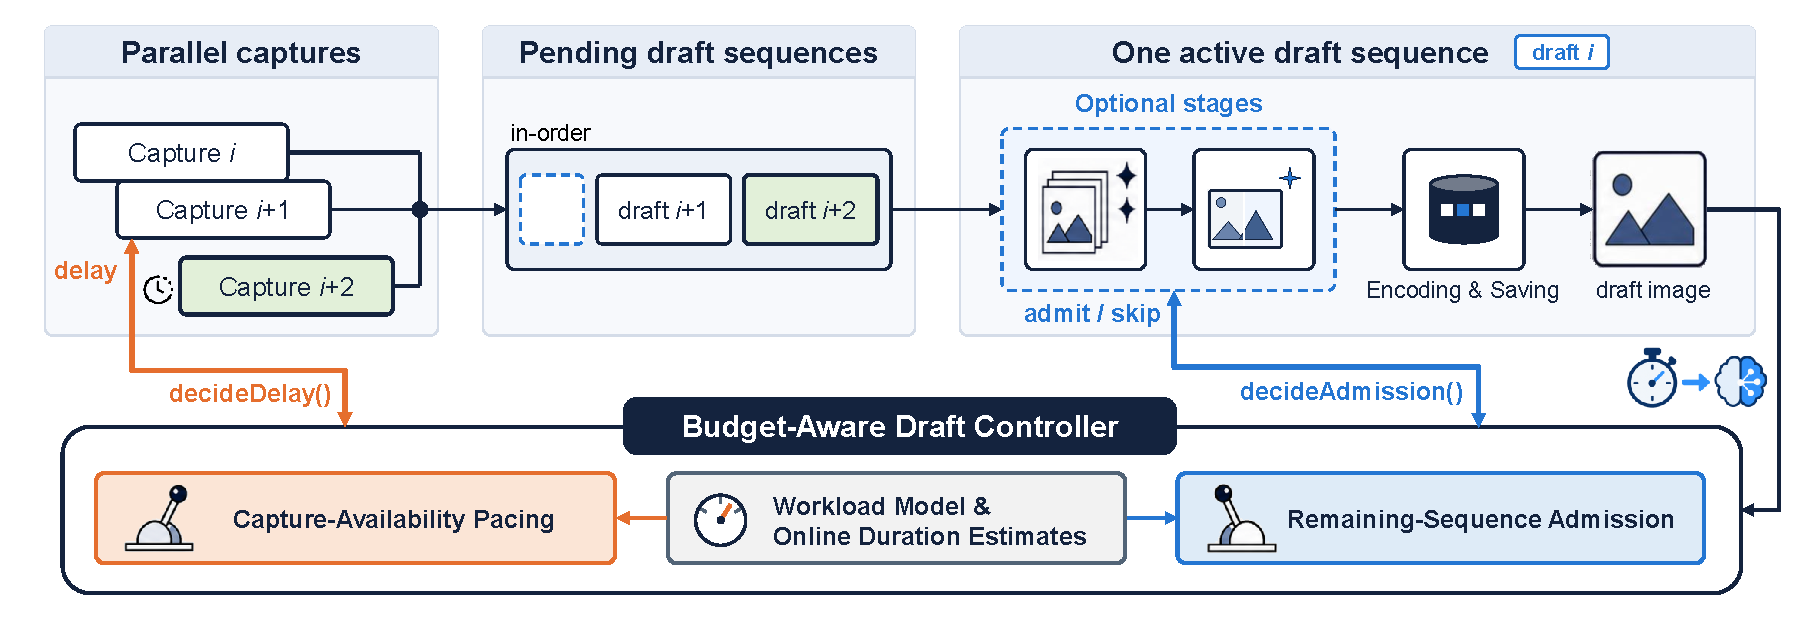
\includegraphics[trim=12 10 0 11,clip,width=\textwidth]{figures/fig_controller_interaction.pdf}
  \caption{Overview of the Budget-Aware Draft Controller.}
  \label{fig:controller-overview}
\end{figure*}
We introduce the \emph{Budget-Aware Draft Controller} to enable lightweight multi-frame composition under parallel capture while meeting each capture's deadline.

\smallskip\noindent\textbf{Controller architecture.}
The controller manages both the work occupying the single draft worker and the requests entering its queue, as shown in Figure~\ref{fig:controller-overview}.
\emph{Remaining-Sequence Admission} runs immediately before an optional stage in the active draft sequence.
It compares the estimated time for the remaining sequence with the capture's remaining timeout budget to decide whether to execute the stage.
\emph{Capture-Availability Pacing} controls delivery of \texttt{captureAvailable}, which exposes the next capture opportunity to the application.
It uses estimated worker occupancy and the remaining deadline window to decide whether to deliver the callback immediately or delay it.

Both modules learn duration estimates from the per-stage and sequence-level measurements of completed draft sequences.
Their shared runtime state connects the two decisions: when admission skips optional stages, pacing adjusts its duration reserve to reflect the stages still eligible for execution.

\smallskip\noindent\textbf{Control objective.}
Capture Timeout is a hard product constraint on enabling optional stages.
Each accepted capture starts its own deadline clock, but its Draft Sequence may wait behind earlier captures on the shared worker.
This waiting consumes the budget available for the remaining stages.
Admission can reduce the remaining processing time by skipping optional stages, but it cannot recover time already spent waiting.
Pacing can delay the next capture opportunity to let the worker progress, but it cannot change work already in progress.
At each decision, the controller compares a processing-time forecast with the live remaining timeout budget.

Within this deadline constraint, the controller prioritizes user-perceived responsiveness.
Capture delay lengthens the shot-to-shot interval and cannot be recovered, whereas the fidelity cost of a skipped stage ends when the final image replaces the draft image.
The controller therefore implements a deadline-constrained, responsiveness-dominant trade-off rather than a global cost optimization.
